\documentclass[12pt,a4paper]{scrartcl}
\usepackage[utf8]{inputenc}
\usepackage[english,russian]{babel}
\usepackage{indentfirst}
\usepackage{misccorr}
\usepackage{graphicx}
\usepackage{amsmath}
\usepackage{multirow}
\usepackage{pgfplots}
\usepackage{slashbox}
\usepackage[top=1cm, bottom=1cm, left=1cm, right=1cm]{geometry}
\pgfplotsset{compat=1.9}

\begin{document}
	\graphicspath{{C:/Users/Alex/OneDrive/Изображения/TexImgs}}
	
	\newcommand{\ms}{\mathstrut}
	\newcommand{\msp}{\hspace{0.5cm}}
	\newcommand{\al}{\alpha}
	\newcommand{\dg}{^\circ}
	\newcommand{\qd}[2]{^{\frac{#1}{#2}}}
	\newcommand{\qdm}[2]{^{-\frac{#1}{#2}}}
	\newcommand{\lm}[2]{\underset{#1 \rightarrow #2}{\lim}}
	\newcommand{\sfrac}[2]{\dfrac{\strut #1}{\strut #2}}
	\newcommand{\equal}[1]{\overset{(#1)}{=}}
	\newcommand{\linevdots}{\ \raisebox{-.08\height}{\vdots}\ }
	\newcommand{\linecvdots}{\ \raisebox{-.08\height}{\vdots}\hspace{-0.13cm}\raisebox{.15\height}{\cancel{\phantom{a}}\hspace{0.06cm}}}
	\newcommand{\combox}[1]{\ms \msp \msp \begin{minipage}{0.95\linewidth}
			#1
	\end{minipage}}
	
	\newtheorem{pr}{Задача}
	\newtheorem{ex}{Пример}
	\newtheorem{dfn}{Def}
	\newtheorem{theorem}{Th}
	
	\newenvironment{slv}{\ms \msp \textit{Решение:}}{}
	\newenvironment{proof}{\ms \msp \textit{Доказательство: }}{\hfill $\square$}
	
	\begin{titlepage}
		
		\vspace*{\fill}
		
		\begin{center}
			
\includegraphics[scale=0.8]{MIPT.png}
			\\[0.7cm]\Huge Московский Физико-Технический Институт\\(национальный исследовательский университет)
			\\[2cm]\LARGE Отчет по эксперименту
			\\[0.5cm]\noindent\rule{\textwidth}{1pt}
			\\\Huge\textbf{Экспериментальная проверка закона вращательного движения\\на крестообразном маятнике}
			\\[-0.5cm]\noindent\rule{\textwidth}{1pt}
		\end{center}
		
		\begin{flushleft}
			\textit{Работа №1.2.2; дата: 26.10.21}\hfill\textit{Семестр: 1}
		\end{flushleft}
		
		\vspace*{\fill}
		
		\begin{flushleft}
			Выполнил: \hspace{\fill} Группа:
			\\Кошелев Александр \hspace{\fill} Б05-105
		\end{flushleft}
	\end{titlepage}
	
	%Страница 2
	
	\begin{flushleft}
		\footnotesize{Экспериментальная проверка закона вращательного движения на крестообразном маятнике} \hspace{\fill} \footnotesize{2}
		\\[-0.3cm]\noindent\rule{\textwidth}{0.3pt}
	\end{flushleft}
	
	\section{Аннотация}
	
	\textbf{Цель работы: } экспериментально проверить закон вращательного движения, получив зависимость углового ускорения от момента инерции и момента прикладываемых к системе сил, а также проанализировать влияние сил трения, действующих в оси
	
	\textbf{Схема установки:}
	\begin{center}
		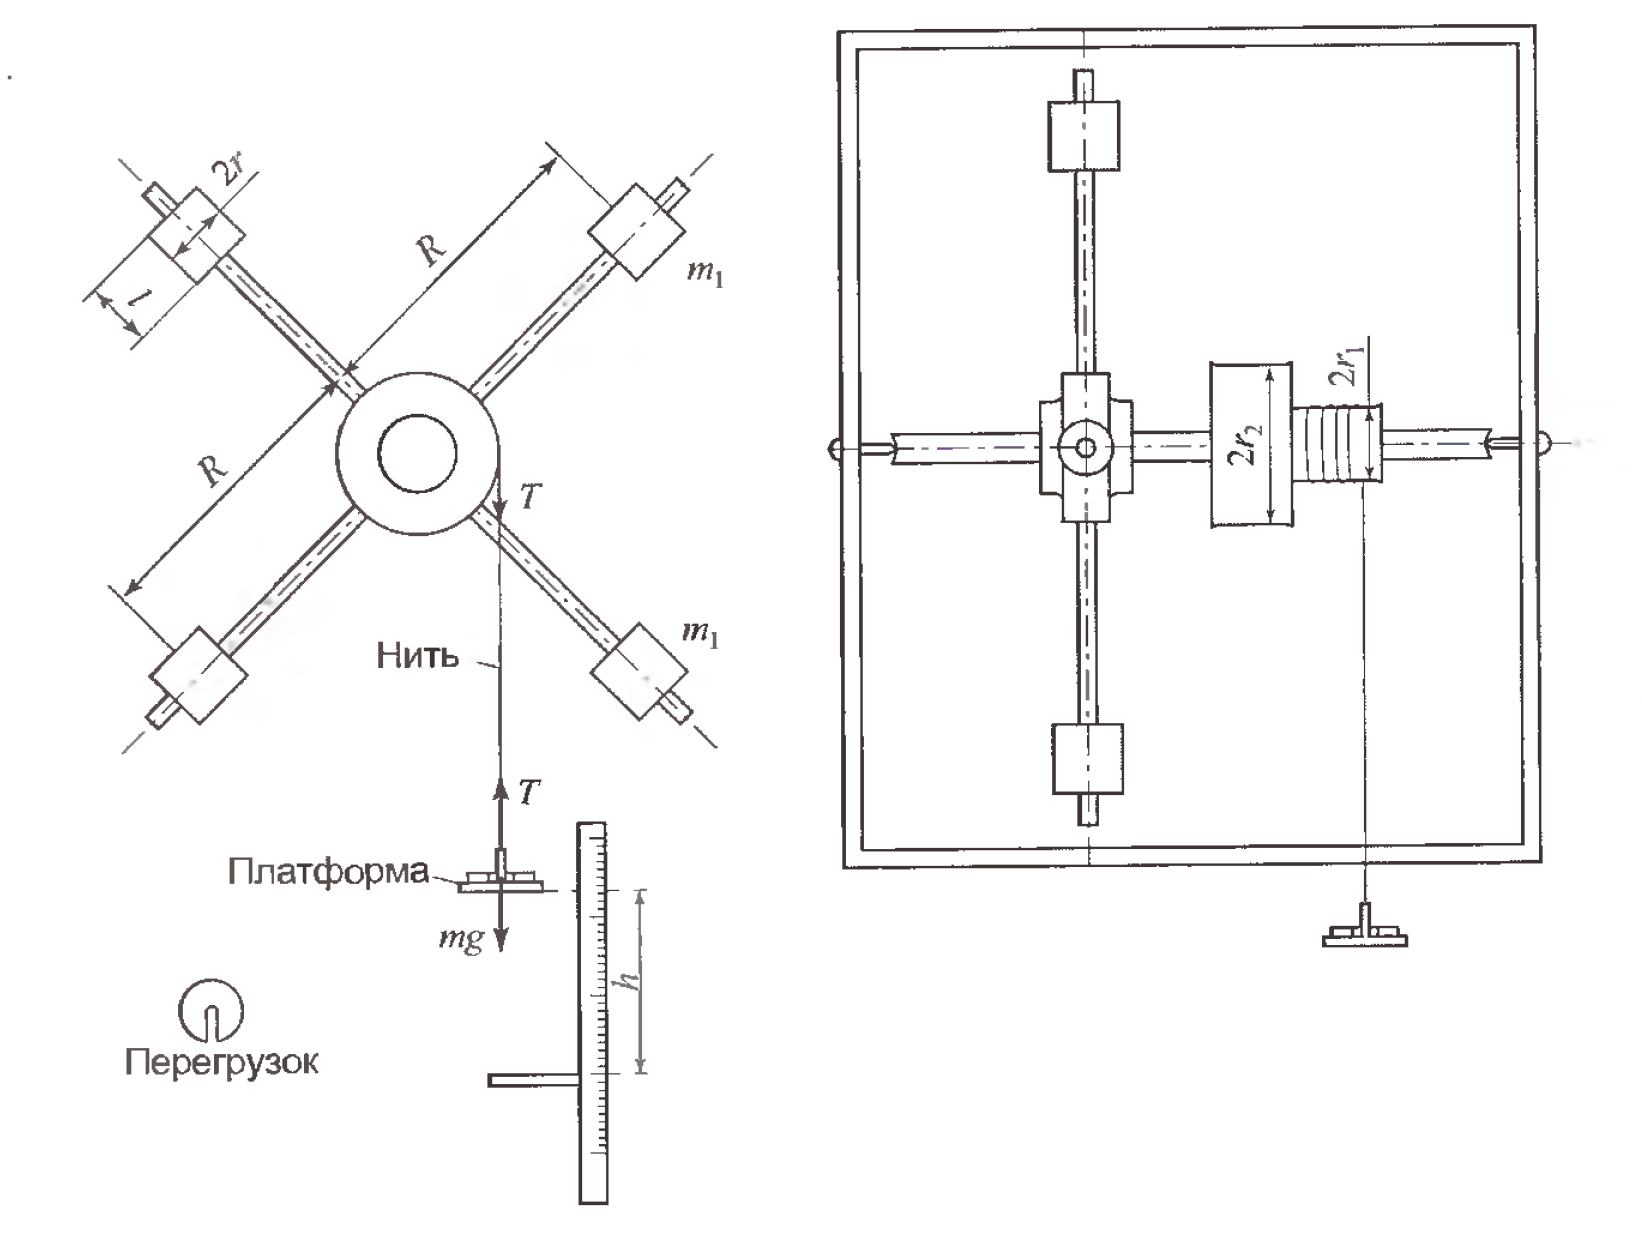
\includegraphics[scale=0.3]{PIC_1.png}
		\\\textbf{Рис. 1:} Схема установки
	\end{center}
		
	Для экспериментального исследования закона вращательного движения в работе используется крестообразный маятник, устройство которого изображено на Рис.1. Маятник состоит из четырёх тонких стержней радиуса $a$, укреплённых на втулке под прямым углом друг к другу. Втулка и два шкива различных радуисов  ($r_1$ и $r_2$) насажены на общую ось. Ось закреплена в подшипниках, так что вся система может свободно вращаться вокруг горизонтальной оси. Момент инерции $I$ маятника можно изменять, передвигая грузы $m_i\ (i = 1, \dots, 4)$ вдоль стержней и меняя $R_i$. На один из шкивов маятника навита тонкая нить. Привязанная к ней лёгкая платформа известной массы $m_{\text{п}}$ служит для размещения перегрузков $m_{\text{г}}$.
	
	Установка оснащена датчиком, позволяющим фиксировать моменты времени прохождения концов стержней через него. Данные с датчика передаются на компьютер для последующей обработки и получения зависимостей угла поворота $\varphi(t)$, угловой скорости $\omega \equiv \dot{\varphi}$ и углового ускорения маятника $\beta \equiv \ddot{\varphi}$ от времени, а также углового ускорения от угловой скорости $\beta(\omega)$.
	
	\section{Теоретические сведения}
	
	 Основное уравнение вращательного движения тела вокруг закреплённой оси:
	 \begin{equation}
	 	I \ddot{\varphi} = M
	 \end{equation}
 
	 где $\ddot{\varphi} \equiv \dot{\omega} \equiv \beta$ -- угловое ускорение ($\omega$  -- угловая скорость), $I$ -- полный момент инерции тела относительно оси вращения, $M$ -- суммарный момент внешних сил относительно этой оси.
	 
	 %Страница 2
	 
	 \newpage
	 
	 \begin{flushleft}
	 	\footnotesize{Экспериментальная проверка закона вращательного движения на крестообразном маятнике} \hspace{\fill} \footnotesize{3}
	 	\\[-0.3cm]\noindent\rule{\textwidth}{0.3pt}
	 \end{flushleft}
 
	Рассмотрим силы, действующие на маятник. Основной вращающий момент поздаётся подвешенным на нити перегрузком. Непосредственно на маятник действует момент силы натяжения нити: $M_{\text{н}} = rT$, где $r$ -- радиус шкива ($r_1$ или $r_2$). Силу $T$ выразим из уравнения движения платформы $m_{\text{н}}\ddot{y}= m_{\text{н}}g - T$, где $m_{\text{н}} = m_{\text{п}} + m_{\text{г}}$ -- масса платформы с перегрузком. Ускорение платформы связано с угловым ускорением маятника условием нерастяжимости нити $\ddot{y}=\beta r$. Отсюда момент силы натяжения нити 
	
	\begin{equation}
		M_{\text{н}} = m_{\text{н}} r(g - \beta r)
	\end{equation}

	Вращению маятника препятствует момент силы трения в оси  $M_{тр}$. Таким образом, с учётом (2) уравнение (1) может быть записано как
	
	\begin{equation}
		I\beta = m_{\text{н}}gr - {M_{тр}}.
	\end{equation}

	Заметим, что в наших опытах, как правило, $m_{\text{н}}r^2 \ll I$, и соответственно $M_{\text{н}} \approx m_{\text{н}}gr$, то маятник будет раскручиваться с постоянным угловым ускорением $\beta _0 \approx m_{\text{н}}gr / I$.
	
	Поскольку зависимость момента силы трения от нагрузки на маятник и скорости его вращения не известна (её исследование -- отдельная экспериментальная задача), методика измерения должна быть построена так, чтобы минимизировать или вовсе исключить влияние $M_{тр}$. Можно высказать следующие качественные соображения о природе и величине $M_{тр}$. Она может иметь как составляющую, пропорциональную силе реакции в оси $N$ (сухое трение в подшипниках),  так и составляющую, пропорциональную угловой скорости $\omega$ вращения маятника (вязкое трение в подшипниках и сопротивления воздуха). Учитывая, что сила реакции уравновешенного маятника равна $N = m_{\text{м}}g + T \approx (m_{\text{м}} + m_{\text{н}})g \approx m_{\text{м}}g $, где $m_{\text{м}}$ -- масса маятника (как правило, $m_{\text{м}} \gg m_{\text{н}}$), можно записать
	
	\begin{equation}
		M_{тр} \approx \left(1 + \frac{m_{\text{н}}}{m_{\text{м}}}\right)M_0 + \eta\omega \approx M_0 + \eta\omega,
	\end{equation}

	где $M_0$ -- момент сил трения для покоящегося маятника при нулевой массе подвеса (минимальное значение силы трения), $\eta$ -- некоторый коэффициент, отвечающий за вязкое трение.
	
	Момент инерции всей системы из теоремы Гюйгенса-Штейнера:
	
	\begin{equation}\label{5}
		I = I_0 + \sum\limits_{i = 1}^4{(I_i + m_i R_i^2)}
	\end{equation}

	где $I_0$ - момент инерции системы без грузов\\
	Момент инерции $i-$того груза относительно оси, проходящей через его центр масс:
	
	\begin{equation}
		I_i = \dfrac{1}{12}m_i h^2 + \dfrac{1}{4}m_i(a_1^2 + a_2^2)    
	\end{equation}

	\section{Проведение эксперимента}
	
	\paragraph{Балансировка маятника} \hfill
	
	\par Будем менять координату грузов, пока маятник не придет в положение безразличного равновесия. Для проверки балансировки необходимо приведем маятник во вращение с небольшой угловой скоростью, дав ему возможность остановиться. Если движение маятника не имеет колебательного характера (является апериодическим), систему можно считать сбалансированной. Кроме того, при быстром вращении несбалансированность маятника может
	быть определена по стуку в оси крепления.
	
	%Страница 4
	
	\newpage
	
	\begin{flushleft}
		\footnotesize{Экспериментальная проверка закона вращательного движения на крестообразном маятнике} \hspace{\fill} \footnotesize{4}
		\\[-0.3cm]\noindent\rule{\textwidth}{0.3pt}
	\end{flushleft}

	Для начала попробуем не нагружать платформу перегрузками и поймем, что момент силы трения покоя $M_0$ мал, так как маятник приходит в движение. Значчит его нельзя определить таким образом. 
	Будем нагружать платформу перегрузками различной массы и заносить в таблицу 1 значения, посчитанные программой Kinematic.
	Для всех измерений $R_1 = 10.1$ см, $R_2 = 10.0$ см, $R_3 = 10$ см, $R_4 = 10$ см. 
	Радиус шкива $r = 1.78$ см.
	Масса платформы $m_{\text{п}} = 15.6$ г. \\
	$\sigma_m = 0.03$ г, $\sigma_r = 0.003$ см.
	$$
	\begin{tabular}[b]{| c | c | c | c |}
		\hline
		$m_{\text{г}}, {\text{г}}$ & $k, 1/c$& $\beta_0, {\text{рад}} / c^2$ & $ M_{\text{н}}, {\text{Н}} \cdot {\text{м}} \cdot 10^{-2} $ \\ \hline
		145.0 & $-0.0213 \pm 0.0041 $ & $    1.689 \pm 0.009 $ & $ 2.80 \pm 0.01 $\\
		100.0 & $ -0.0216 \pm 0.0043 $ & $   1.237 \pm 0.008 $ & $ 2.02 \pm 0.01 $\\
		200.0 & $ -0.02449 \pm 0.0037 $ & $  2.325 \pm 0.009 $ & $ 3.76 \pm 0.01 $ \\
		50.3 & $-0.0201 \pm 0.0040 $ & $     0.693 \pm 0.006 $ & $ 1.15 \pm 0.01 $\\
		126.4 & $ -0.0197 \pm 0.0029 $ & $   1.484 \pm 0.006 $ & $ 2.48 \pm 0.01 $\\
		88.4 & $ -0.0163 \pm 0.0024 $ & $    1.055 \pm 0.003 $ & $ 1.82 \pm 0.01 $\\
		188.4 & $ -0.0147 \pm 0.0018 $ & $   2.136 \pm 0.003 $ & $ 3.56 \pm 0.01 $\\
		162.0 & $ -0.0236 \pm 0.0017 $ & $   1.889 \pm 0.004 $ & $ 3.10 \pm 0.01 $ \\
		45.0 & $ -0.0246 \pm 0.0045 $ & $    0.378 \pm 0.005 $ & $ 1.06 \pm 0.01 $\\ \hline
	\end{tabular}
	$$
	\begin{center}
		\textbf{Табл. 1: } Значения $\beta_0$, $k$, посчитанные программой и $M_{\text{н}}$ 
	\end{center}

	По результатам измерений и посчитанным значениям из таблицы 1 построим график $\beta_0(M_{\text{н}})$. \\
	
	\begin{center}
		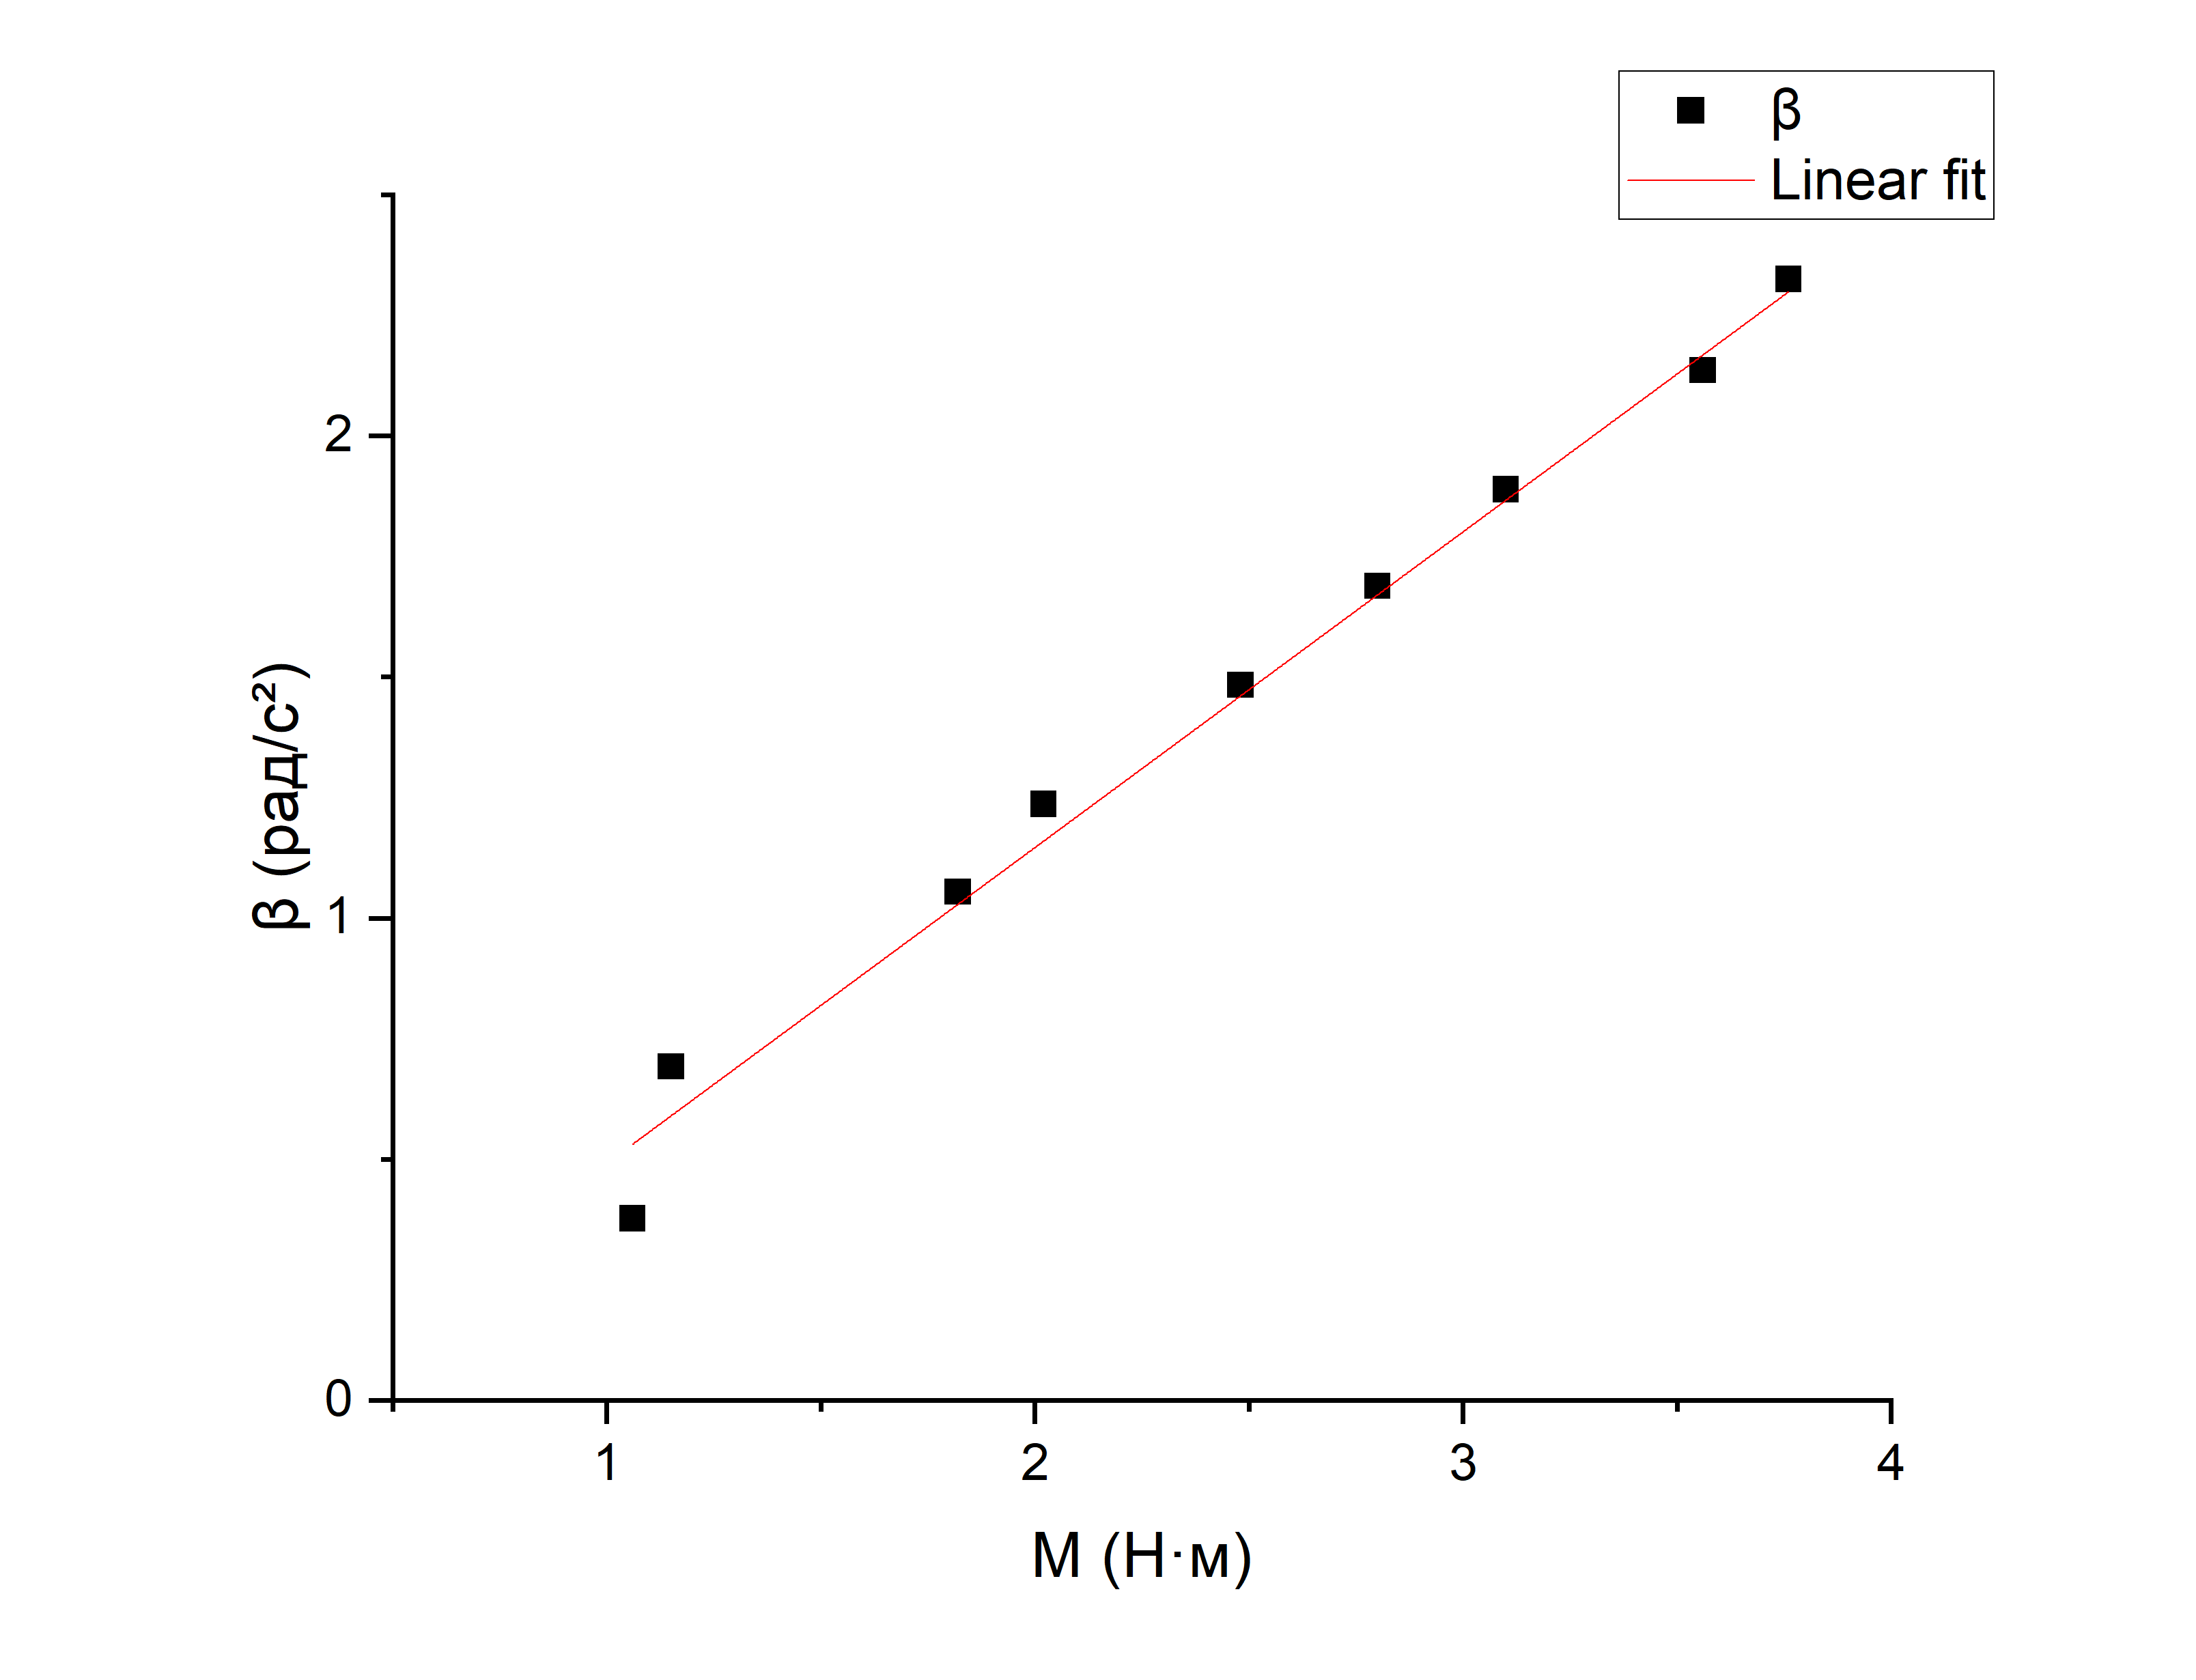
\includegraphics[scale=0.5]{PIC_2.png}
		\\\textbf{Рис.2 :} График зависимости $\beta_0(M_{\text{н}})$
	\end{center}
	
	Пользуясь линейной аппроксимацией, можем найти коэффициенты прямой $\beta_0 = \gamma M_{\text{н}} + b$: 
	
	$$\gamma = 66.3 \pm 0.3\,(\text{кг}\cdot\text{м}^2)^{-1}$$
	$$b = - 0.16 \pm 0.07\, \text{рад/с}^2$$
	
	 то есть $M_0 = -b / \gamma = 0.0024 \pm 0.007$ Н $\cdot$ м (пересечение с осью). $M_0$ действительно оказался мал, так как $M_0 \ll m_{\text{н}}gr$, что и было заявлено изначально.
 
 	%Страница 5
 	
 	\newpage
 	
 	\begin{flushleft}
 		\footnotesize{Экспериментальная проверка закона вращательного движения на крестообразном маятнике} \hspace{\fill} \footnotesize{5}
 		\\[-0.3cm]\noindent\rule{\textwidth}{0.3pt}
 	\end{flushleft}
 	
 	\paragraph{Измерения при различном расстоянии до грузов} \hfill
 	
 	\par Будем менять координату грузов при постоянной массе перегрузка $m = 145$ г, занося в Табл. 2 значения, посчитанные программой Kinematic, а также координаты грузов. \\
 	Массы грузов $m_1 = 146.5$ г, $m_2 = 146.6$ г, $m_3 = 146.6$ г, $m_4 = 150.2$ г. Также из уравнения (3) найдем $I$.
 	
 	$$
 	\begin{tabular}[b]{| c | c | c | c | c | c | c | c |}
 		\hline
 		$R_1, \text{см}$ & $R_2, \text{см}$ & $R_3, \text{см}$ & $R_4, \text{см}$ & $R, \text{см}$ & $k, 1/c$ & $\beta_0, {\text{рад}} / c^2$ & $I, \text{кг} \cdot \text{м}^2 \cdot 10^{-2} $\\ \hline
 		10.1 & 10.2 & 10.0 & 10.0 & 10.1 & $ -0.0246 \pm 0.0045 $ & $ 1.741 \pm 0.009 $ & $1.30 \pm 0.01$ \\
 		8.0 & 8.0 & 8.0 & 7.6 & 7.9 &     $ -0.0217 \pm 0.0025 $ & $ 2.156 \pm 0.006 $ & $1.05 \pm 0.01$ \\
 		5.7 & 5.7 & 5.8 & 5.3 & 5.6 &      $ -0.0340 \pm 0.0031 $ & $ 2.786 \pm 0.008 $ & $0.81 \pm 0.01$ \\
 		5.2 & 4.7 & 5.0 & 4.2 & 4.8 &      $ -0.0367 \pm 0.0081 $ & $ 3.043 \pm 0.028 $ & $0.74 \pm 0.02$ \\ 
 		12.1 & 12.2 & 12.3 & 11.5 & 12.0 & $ -0.0189 \pm 0.0036 $ & $ 1.486 \pm 0.007 $ & $1.52 \pm 0.01$ \\ 
 		\hline
 	\end{tabular}
 	$$
 	\begin{center}
 		\textbf{Табл. 2: } Момент инерции системы в зависимости от координаты грузов
 	\end{center}
 
 	По значениям из Табл. 2 и полученным ранее значениям построим график зависимости $I(R^2)$:
 	
 	\begin{center}
 		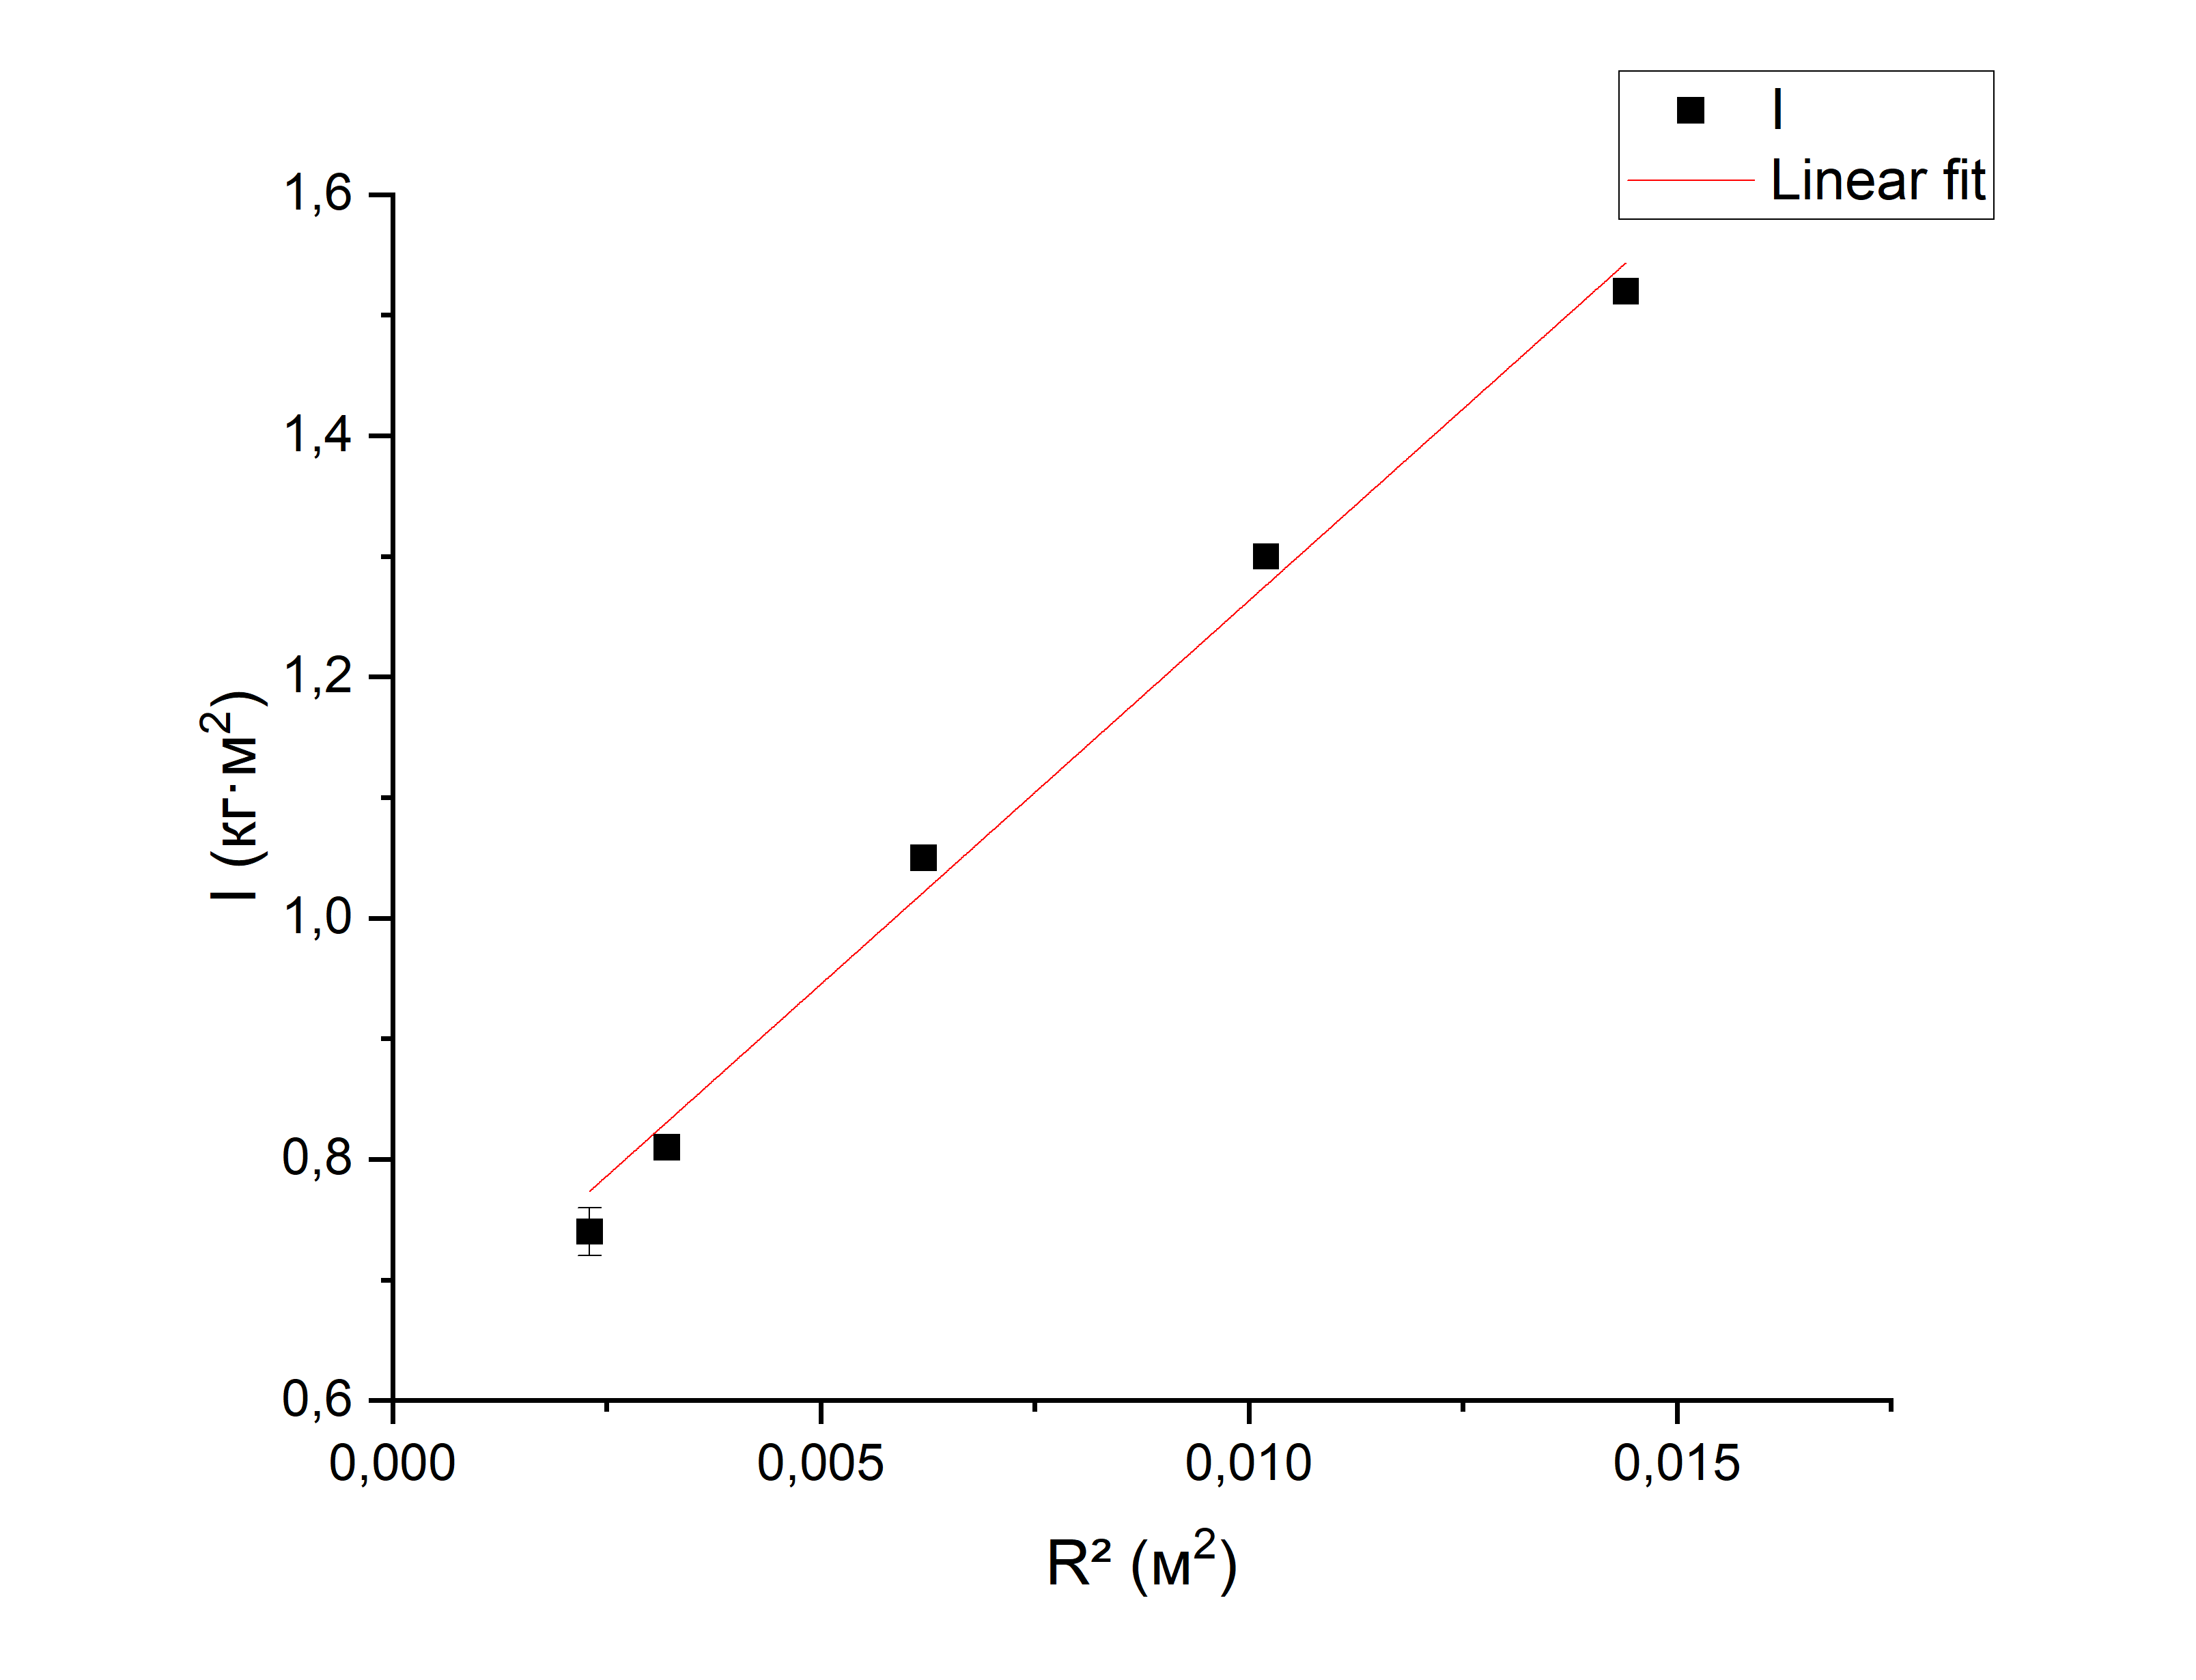
\includegraphics[scale=0.5]{PIC_3.png}
 		\\\textbf{Рис. 3: } График зависимости $I(R^2)$
 	\end{center}
 	
 	Из этого графика можно найти момент инерции пустого маятника. Для этого при помощи линейной аппроксимации найдем значение в нуле и вычтем моменты инерции грузиков. Поскольку значения $I_i$ примерно равны, можно считать, что $\sum\limits_{i = 1}^4{(I_i + m_i R_i^2)} \approx 4I_1 = 4.875 \cdot 10^{-5}$ кг $\cdot$ м$^2$. Тогда:
 	
 	$$I_0 = (0,627 \pm 0,029) \cdot 10^{-2}\,\text{кг}\cdot\text{м}^2$$
 	
 	\paragraph{Прямое измерение момента инерции пустого маятника} \hfill
 	
 	\par Проведем серию измерений без грузов, чтобы найти $I_0$, и занесем результат в Табл. 3.
 	
 	%Страница 6
 	
 	\newpage
 	
 	\begin{flushleft}
 		\footnotesize{Экспериментальная проверка закона вращательного движения на крестообразном маятнике} \hspace{\fill} \footnotesize{6}
 		\\[-0.3cm]\noindent\rule{\textwidth}{0.3pt}
 	\end{flushleft}
 	
 	$$
 	\begin{tabular}[b]{| c | c | c | c |}
 		\hline
 		$m_{\text{н}}, \text{г} $ & $k, 1/c$ & $\beta_0, \text{рад}/ \text{с}^2$ & $I_0, \text{кг} \cdot \text{м}^2 \cdot 10^{-2} $\\ \hline
 		115,6 & $ -0.0551 \pm 0.0061 $ & $ 3.517 \pm 0.017 $ & $0.574 \pm 0.018$ \\
 		166.9 & $ -0.0654 \pm 0.0066 $ & $ 5.098 \pm 0.022 $ & $0.572 \pm 0.022$ \\
 		78.5 &  $ -0.0453 \pm 0.0048 $ & $ 2.391 \pm 0.021 $ & $0.573 \pm 0.021$ \\
 		215.6 & $ -0.0747 \pm 0.0053 $ & $ 6.748 \pm 0.020 $ & $0.568 \pm 0.020$ \\
 		185.7 & $ -0.0709 \pm 0.0030 $ & $ 5.676 \pm 0.011 $ & $0.571 \pm 0.011$ \\ \hline
 	\end{tabular}
 	$$
 	\begin{center}
 		\textbf{Табл. 3: } Измерение момента инерции пустого маятника
 	\end{center}
 
 	Из Табл. 3 получаем:
 	
 	$$I_0 = (0.572 \pm 0.022) \cdot 10^{-2}\,\text{кг}\cdot\text{м}^2$$
 	
 	Этот результат удовлетворительно согласуется с результатом, полученном в предыдущем пункте.
 	
 	\section{Выводы}
 	
 	Мы убедились, что угловое ускорение маятника обратно пропорционально моменту инерции тела и прямо пропорционально моменту прикладываемых сил, то есть уравнение (1) верно. Помимо этого было выяснено, какой вклад в общий момент сил вносит момент силы трения в оси вращения -- этот вклад мал, как и было предположенно изначально. Также несколькими способами была найдена величина момента инерции самого маятника, и получены следующие результаты:
 	
 	$$I_0 = (0,627 \pm 0,029) \cdot 10^{-2}\,\text{кг}\cdot\text{м}^2$$
 	$$I_0 = (0.572 \pm 0.022) \cdot 10^{-2}\,\text{кг}\cdot\text{м}^2$$
 	
 	Данные результаты удовлетворительно совпадают в пределах одной величины погрешности. 	
\end{document} 	